\chapter{A Case study of legged locomotion}
\label{sec:casestudy}


\section{Requirement of legged locomotion}
\label{sec:case_req}

\subsection{Fast leg placement}
\label{sec:fast}

\subsection{Impact management}
\label{sec:impact}

\subsection{High load bearing}
\label{sec:load}


\section{Solution based on variable gear-ratio actuators}
\label{sec:case_sol}

\begin{figure}[H]
        \centering
				\subfloat[Fast leg placement]{
				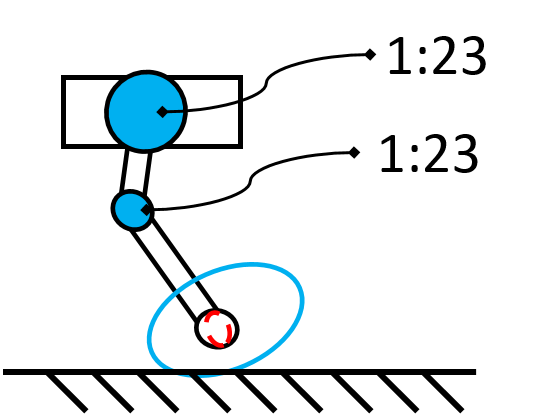
\includegraphics[width=0.35\textwidth]{legHS.png}
				\label{fig:legHS}}
        \subfloat[High load bearing]{
				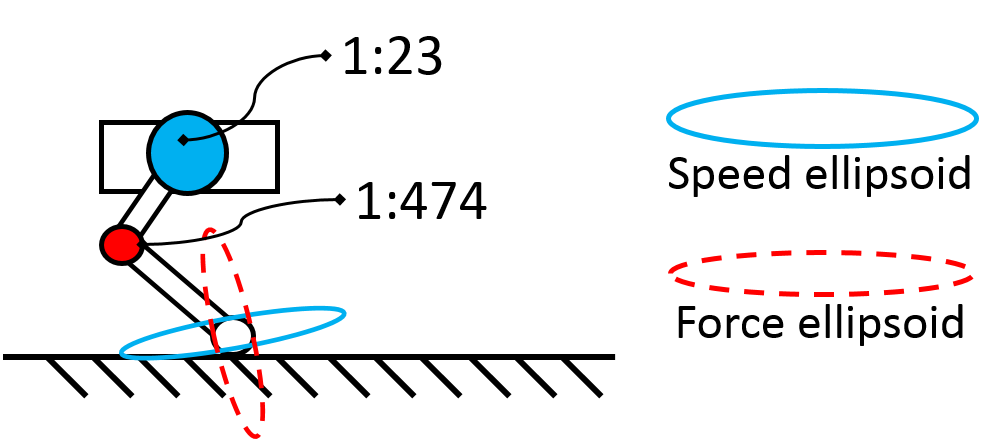
\includegraphics[width=0.65\textwidth]{legHF.png}
				\label{fig:legHF}}
        \caption{Advantageous gear-ratio selection for locomotion}\label{fig:legsol}
\end{figure}



\section{Case Study: 1-DoF leg landing}

\subsection{Modeling}

\begin{figure}[htp]
	\centering
		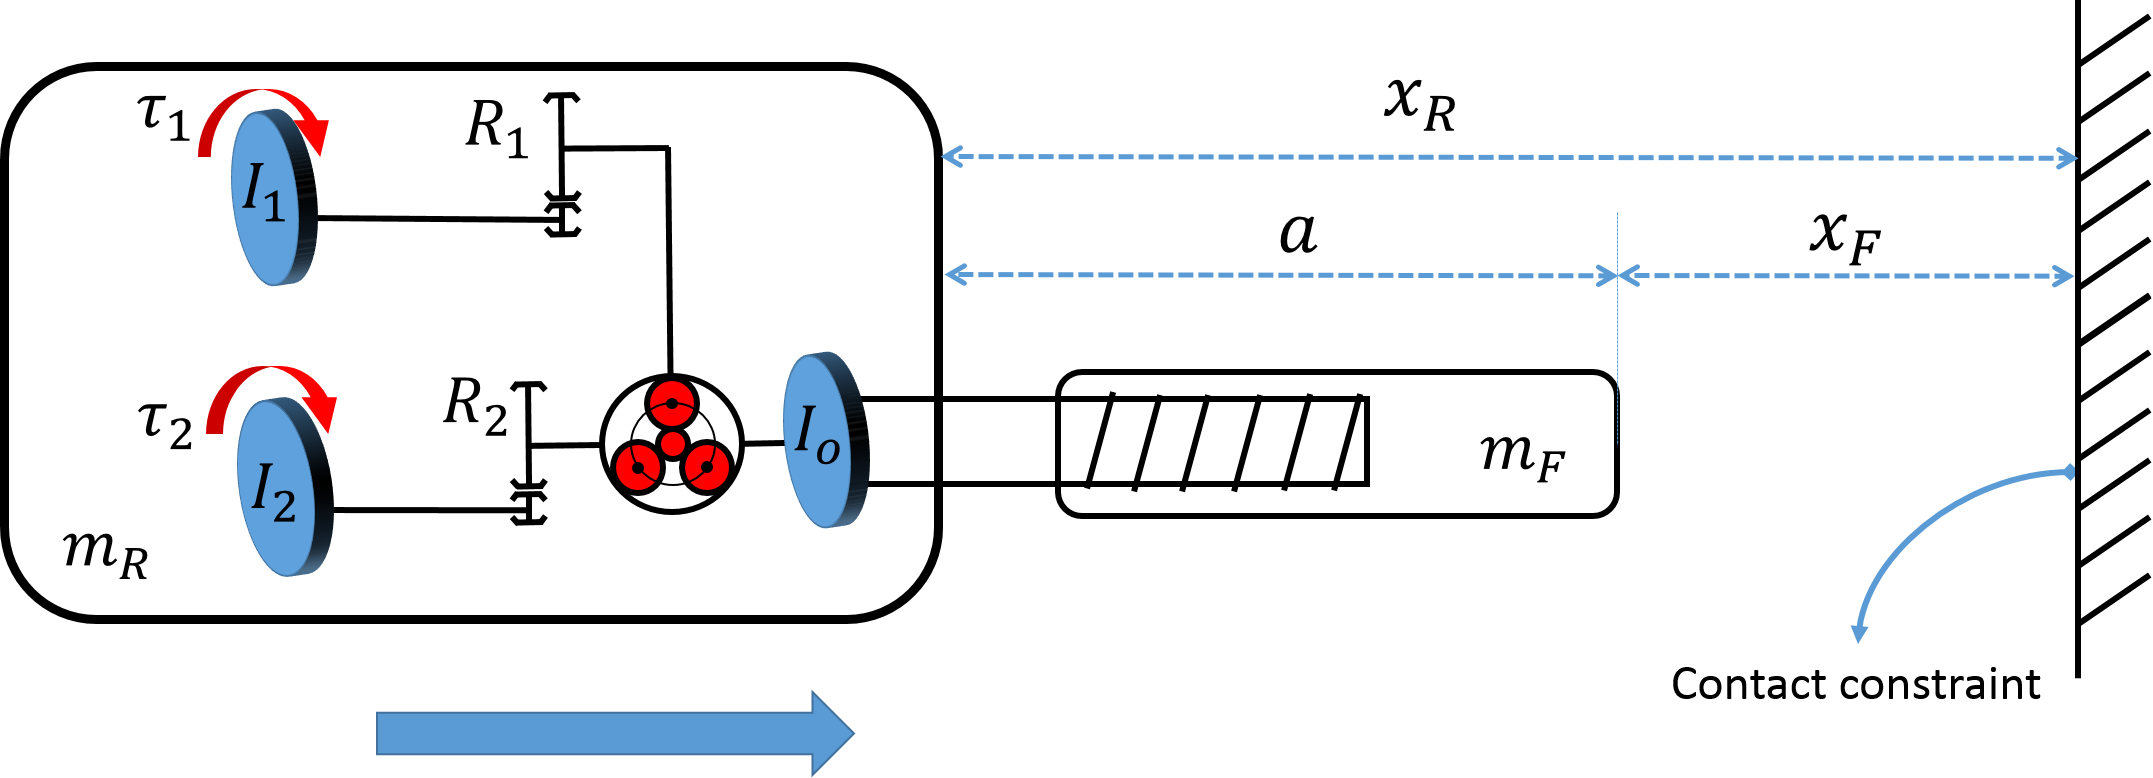
\includegraphics[width=0.95\textwidth]{1dof_landing.png}
	\caption{Simple Robot Landing with a 1-DoF leg equipped with a DSDM}
	\label{fig:1dof_landing}
\end{figure}

Presence of M2 DoF neglected.

Kinematic:

\begin{align}
\text{actuator output relative velocity} : \dot{a} 
\end{align}

Kinetic energy:

\begin{align}
T &= 1/2 \left[ m_R \right] \dot{x}_R^2 + 1/2 \left[ m_F \right] \dot{x}_F^2 + 1/2 \underbrace{\left[ I_o + R_1^2 I_1 \right]}_{I_a} \dot{a}^2 \\
T &= 1/2 
\left[ \begin{array}{c c}
\dot{x}_R & \dot{a}
\end{array} \right] 
\underbrace{
\left[ \begin{array}{c c}
m_R + m_F & -m_F \\
-m_F      & I_a + m_F
\end{array} \right] }_{H}
\underbrace{
\left[ \begin{array}{c}
\dot{x}_R \\ \dot{a}
\end{array} \right] }_{\dot{\vec{q}}}
\end{align}

Generalized forces:





Contact constraint:

%
\begin{align}
\phi( \vec{q} )       &= x_R - a = 0 \\
\dot{\phi}( \vec{q} ) &= J_c\vec{\dot{q}}  = 0 \\
J_c                   &= \frac{d \phi}{d\vec{q}} = \left[ \begin{array}{c c} 1 & -1 \end{array} \right]
\label{eq:dsdm_impact_const}
\end{align}


%
EoM:


\begin{align} 
\underbrace{
\left[ \begin{array}{c c}
m_R + m_F & -m_F \\
-m_F      & I_a + m_F
\end{array} \right] }_{H}
\underbrace{
\left[ \begin{array}{c}
\ddot{x}_R \\ \ddot{a}
\end{array} \right] }_{\ddot{\vec{q}}}
+
\underbrace{
\left[ \begin{array}{c c}
0      & 0 \\
0      & b_a 
\end{array} \right] }_{D}
\underbrace{
\left[ \begin{array}{c}
\dot{x}_R \\ \dot{a}
\end{array} \right] }_{\dot{\vec{q}}}
+
\underbrace{
\left[ \begin{array}{c}
-(m_R+m_F)g \\ m_F g 
\end{array} \right] }_{\vec{g}}
=
\underbrace{
\left[ \begin{array}{c}
0 \\ R_1
\end{array} \right] }_{B}
\tau_1
+
\underbrace{
\left[ \begin{array}{c}
1 \\ -1
\end{array} \right] }_{J_c^T}
f_c
\end{align}


%
Ground contact force
%
\begin{align}
\int{  f_c dt } &= - \left( J_c H^{-1} J_c^T \right)^{-1}  J_c \vec{\dot{q}}^- =
\left[ m_F + (\frac{m_R I_a}{m_R + I_a}) \right] \underbrace{(\dot{x}_R^- - \dot{a}^-)}_{\dot{x}_F^-}
\label{eq:dsdm_impact_force}
\end{align}
%
Changes in velocity
%
\begin{align}
\left[ \begin{array}{c}
\Delta \dot{x}_R \\ \Delta \dot{a}
\end{array} \right]
 &= H^{-1} J_c^T \int{  f_c dt } = \frac{1}{I_a + m_R} \left[ \begin{array}{c}
I_a \\ -m_R
\end{array} \right] \dot{x}_F^-
\label{eq:dsdm_impact_delta}
\end{align}
%


\subsection{Flight Phase Control}

\subsubsection{High-level Robot Controller}

Under-actuated and uncontrollable


Reduced system for partial feedback linearization:
\begin{align}
\left[ I_a + \left( \frac{m_F m_R}{m_F + m_R} \right) \right] \ddot{a} + \Bigg[ b_a \Bigg] \dot{a} = R_1 \tau_1 \\
\frac{1}{R_1}
\underbrace{\left(
\left[ I_o + \left( \frac{m_F m_R}{m_F + m_R} \right) \right] \ddot{a} + \Bigg[ b_o \Bigg] \dot{a}
\right)}_{\tau_E}
+ R_1
\underbrace{\left(
 I_1 \ddot{a} + b_1 \dot{a}
\right)}_{\tau_I}
= \tau_1
\end{align}


\subsubsection{Predictive Impact Controller in DSDM Nullspace}


Effect on DSDM actuator.\\
High-level analysis give impulsive behavior of the actuator output DoF:
%
\begin{align}
\Delta \dot{a} = \frac{ \int{\tau_c dt} }{ I_a }  = \frac{-m_R}{I_a + m_R} \dot{x}_F^-
\end{align}
%
Impulsive torque on actuator output:
%
\begin{align}
\int{\tau_c dt} = \frac{-m_R I_a}{I_a + m_R} \dot{x}_F^-
\end{align}
%
Ideal desired M1 velocity before the impact:
\begin{align}
w_{1,d}  = - R_1 \frac{\int{\tau_c dt}}{I_a} =  R_1 \frac{m_R}{I_a + m_R} \dot{x}_F^-
\end{align}
%
Hence if $w_1$ is tracking this target velocity, function of the foot velocity, then after the foot touch the ground:
\begin{align}
w_{1}^+  = 0
\end{align}
and high-force mode can be engaged seamlessly.


\subsection{Ground Phase Control}



\section{Experiments}
\label{sec:case_exp}



